\newpage
\section{Восстановление объектных структур данных при декомпиляции с использованием информации о типах времени выполнения}\label{chapter:reconstruction_with_rtti}

\subsection{Информация о типах времени выполнения в Си++}\label{chapter:rtti_in_cpp}
Обзор существующих решений проблемы восстановления объектных структур данных показал, что с использованием информации о типах времени выполнения возможно восстановление иерархии полиморфных классов в программах на языке Си++ из ассемблерного представления. Информация о типах времени выполнения, или RTTI, используется в языке Си++ для реализации следующих средств \cite{cpp03}:

\begin{itemize}
\item Оператор \lstinline{dynamic_cast<>}. Этот оператор используется для приведения типов, однако в отличие от приведения типов в стиле Си, проверка на корректность производится во время выполнения программы, а не во время компиляции. Обычно этот оператор используется для <<нисходящего>> приведения типов в иерархии классов --- от базового класса к производному. При этом выполняется проверка на то, что переданный объект действительно является экземпляром нужного производного класса. Для реализации такой проверки необходимо на этапе времени выполнения обладать информацией о структуре иерархии классов.

    Еще один способ использования оператора \lstinline{dynamic_cast<>} --- это преобразование к типу \lstinline{void*}. При этом, в отличие от обычного приведения типов, возвращается указатель на начало объемлющего объекта, который в случае множественного наследования может не совпадать с указателем на текущий объект.

\item Оператор \lstinline{typeid}. Этот оператор можно применять к выражениям любого типа, но чаще всего он используется для определения фактического класса переданного объекта во время выполнения. Он возвращает объект типа \lstinline{type_info}, с использованием которого можно, в частности, получить строковое представление имени рассматриваемого класса.

\item Исключительные ситуации. При обработке исключительных ситуаций необходимо сравнивать тип возбужденной исключительной ситуации с типом, указанным в \lstinline{catch}-блоке. Стандарт Си++ не оговаривает детали реализации обработки исключительных ситуаций, однако так как для таких проверок на этапе времени выполнения также может потребоваться информация о структуре иерархии классов, то современные компиляторы зачастую используют приемы, схожие с используемыми в реализации информации о типах времени выполнения. К примеру, Компилятор MSVC для каждого \lstinline{catch}-блока хранит объекты типа \lstinline{type_info}, соответствующие всем типам исключительных ситуаций, которые могут быть обработаны данным \lstinline{catch}-блоком, а согласно стандарту Си++, эти типы находятся в одной иерархии наследования \cite{kochhar02}.
\end{itemize}

В стандарте Си++ описан интерфейс этих средств, но ничего не сказано о том, как они должны быть реализованы. Их реализация зависит от используемого компилятором \textit{бинарного интерфейса приложений}.

Бинарный интерфейс приложений для Си++ кроме формата информации и типах времени выполнения также определяет используемые {\it соглашения о вызовах}, схему {\it декорирования имен} и некоторые другие детали. В частности, бинарный интерфейс приложений определяет способ реализации виртуальных функций. В современных компиляторах для Си++ этот механизм реализован следующим образом: для каждого полиморфного класса генерируется \textit{таблица виртуальных функций}, содержащая указатели на все виртуальные методы класса. Каждый объект такого класса хранит указатель на соответствующую таблицу, и все вызовы виртуальных функций производятся косвенно, с использованием этого указателя, что называется {\it поздним связыванием} \cite{gray94, gccabi}.

Рассмотрим бинарный интерфейс приложений, используемый в компиляторах GCC и MSVC для платформы x86.

Как компилятор GCC, так и компилятор MSVC генерируют информацию о типах времени выполнения для всех используемых в приложении полиморфных классов, добавляя указатель на соответствующую классу структуру, содержащую информацию о типах времени выполнения, перед его таблицей виртуальных функций \cite{skochinsky06, gccabi}. Так как каждый экземпляр полиморфного класса и так содержит указатель на таблицу виртуальных функций, то при такой организации компиляция с поддержкой информации о типах времени выполнения не приводит к появлению дополнительных издержек для кода, который информацию о типах времени выполнения не использует.

Рассмотрим формат структур, содержащих информацию о типах времени выполнения, используемый в компиляторах GCC и MSVC.






\subsubsection{Формат информации о типах времени выполнения, используемый в компиляторе MSVC}\label{chapter:rtti_in_msvc}
Компилятор MSVC при использовании информации о типах времени выполнения для каждого полиморфного класса генерирует несколько структур, которые впоследствии используется реализацией механизма обработки исключений и оператором \lstinline{dynamic_cast<>}. Эти структуры не документированы компанией Microsoft, и их формат был восстановлен с использованием методов обратного проектирования. Описание этих структур можно, к примеру, посмотреть в исходных кодах системы Wine, позволяющей пользователям UNIX-подобных операционных систем исполнять приложения, созданные для операционной системы Microsoft Windows \cite{wine}.

Компилятор MSVC для каждого полиморфного класса перед таблицей виртуальных функций помещает указатель на \lstinline{RTTICompleteObjectLocator}, содержащий в частности указатель на структуру \lstinline{RTTIClassHierarchyDescriptor}, описание которой представлено на рис. \ref{listing:rtticlasshierarchydescriptor}.

\begin{figure}[htb!]
\hspace{2cm}
\begin{minipage}[b]{1cm}
\begin{cplusplus}
struct RTTIClassHierarchyDescriptor {
  /** #\tl{Всегда ноль.}@ */
  unsigned long signature;
  
  /** #\tl{Атрибуты, отвечающие за множественное и}@
   * #\tl{виртуальное наследование.}@ */
  unsigned long attributes;
  
  /** #\tl{Количество классов в pBaseClassArray.}@ */
  unsigned long numBaseClasses;
  
  /** #\tl{Указатель на массив структур, описывающих}@ 
   * #\tl{базовые классы.}@ */
  RTTIBaseClassDescriptor** pBaseClassArray;
};
\end{cplusplus}
\end{minipage}
\caption{Описание структуры \lstinline{RTTIClassHierarchyDescriptor}.}
\label{listing:rtticlasshierarchydescriptor}
\end{figure}

Базовые классы задаются структурами типа \lstinline{RTTIBaseClassDescriptor}, описание которой представлено на рис. \ref{listing:rttibaseclassdescriptor}.

\begin{figure}[htb!]
\hspace{2cm}
\begin{minipage}[b]{1cm}
\begin{cplusplus}
struct RTTIBaseClassDescriptor {
  /** #\tl{Указатель на соответствующий объект type\_info.}@ */
  std::type_info* pTypeInfo;
  
  /** #\tl{Количество последующих записей в массиве,}@
   * #\tl{соответствующих классам, являющимся предками}@
   * #\tl{данного.}@ */
  unsigned long numContainedBases;
  
  /** #\tl{Информация для создания указателей на член класса.}@ */
  struct PMD {
    /** #\tl{Смещение члена класса.}@ */
    int mdisp;
    
    /** #\tl{Смещение указателя на таблицу виртуальных базовых}@
     * #\tl{классов.}@ */
    int pdisp;
    
    /** #\tl{Смещение внутри таблицы виртуальных базовых}@
     * #\tl{классов.}@ */
    int vdisp;
  } where;
  
  /** #\tl{Атрибуты, обычно равны нулю.}@ */
  unsigned long attributes;
};
\end{cplusplus}
\end{minipage}
\caption{Описание структуры \lstinline{RTTIBaseClassDescriptor}.}
\label{listing:rttibaseclassdescriptor}
\end{figure}

Описанные выше структуры помещаются в сегмент данных только для чтения. Зная точное расположение этих структур, можно восстановить полную иерархию полиморфных классов приложения. Кроме того, для каждого полиморфного класса генерируется соответствующий объект типа \lstinline{std::type_info}, описание которого представлено на рис. \ref{listing:msvc_type_info}.

\begin{figure}[htb!]
\hspace{2cm}
\begin{minipage}[b]{1cm}
\begin{cplusplus}
class type_info {
public:
  /* ... */
private:
  void *_m_data;
  char _m_d_name[1];
  /* ... */
};
\end{cplusplus}
\end{minipage}
\caption{Описание класса \lstinline{std::type_info}, используемого компилятором MSVC.}
\label{listing:msvc_type_info}
\end{figure}

В поле \lstinline{_m_d_name} записано {\it декорированное} имя класса, соответствующего данному объекту класса \lstinline{std::type_info}. В компиляторе MSVC используется разработанная компанией Microsoft и не опубликованная схема декорирования имен. Как и в случае с форматом структур, содержащих информацию о типах времени выполнения, алгоритм декорирования был восстановлен с использованием методов обратного проектирования \cite{seonghoon06}. Таким образом, используя информацию о типах времени выполнения, можно восстановить полную иерархию полиморфных классов вместе с их именами. Согласно поставленным в главе \ref{chapter:problem} условиям, рассматриваемая программа перед компиляцией не была подвергнута обфускации, то есть восстановленные имена классов соответствуют их реальным именам в исходной программе на языке Си++. При проектировании объектно-ориентированных систем классам стараются давать осмысленные имена, соответствующие их функциональности, и потому знание этих имен может существенно упростить понимание принципов работы системы.




\subsubsection{Формат информации о типах времени выполнения, используемый в компиляторе GCC}\label{chapter:rtti_in_gcc}
\begin{figure}[htb!]
\centering
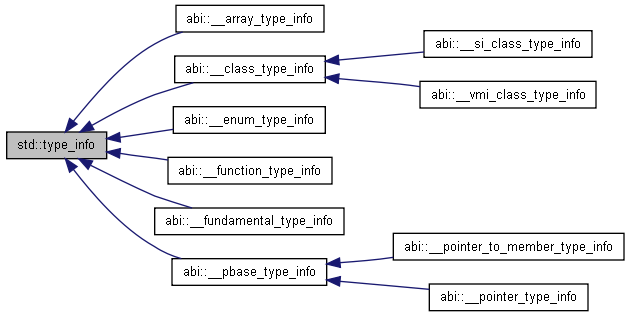
\includegraphics[width=0.9\textwidth]{images/gcc_rtti_hierarchy.png}
\caption{Иерархия производных от \lstinline{std::type_info} классов, используемая в компиляторе GCC.}
\label{fig:gcc_rtti_hierarchy}
\end{figure}


Компилятор GCC, в отличие от MSVC, для хранения информации о типах времени выполнения использует иерархию производных от \lstinline{std::type_info} классов. Описание иерархии этих классов приводится в заголовочном файле \lstinline{<cxxabi.h>}, поставляемом с компилятором GCC, и доступно для использования из любой программы, написанной на Си++. Организация доступа к информации о типах времени выполнения в компиляторе GCC схожа с используемой в MSVC --- для каждого полиморфного класса перед таблицей виртуальных функций помещается указатель на соответствующий ему объект производного от \lstinline{std::type_info} класса, хранящий информацию о типе. Иерархия производных от \lstinline{std::type_info} классов представлена на рис. \ref{fig:gcc_rtti_hierarchy}.

Для классов, не имеющих базовых, используются тип \lstinline{abi::__class_type_info}, не содержащий никакой дополнительной информации по сравнению с \lstinline{std::type_info}. Он является базовым для двух других классов --- \lstinline{abi::__si_class_type_info} и \lstinline{abi::__vmi_class_type_info}. Первый используется для классов, имеющих ровно один невиртуальный публичный базовый класс\footnote{англ. non-virtual public base class --- базовый класс, унаследованный с модификатором \lstinline{public} и без модификатора \lstinline{virtual}.}. По сравнению с \lstinline{std::type_info}, он содержит только одно дополнительное поле - указатель на \lstinline{abi::__class_type_info} соответствующего базового класса. Для всех прочих классов используется тип \lstinline{abi::__vmi_class_type_info}. Описание этого класса представлено на рис. \ref{listing:__vmi_class_type_info}.

\begin{figure}[htb!]
\hspace{2cm}
\begin{minipage}[b]{1cm}
\begin{cplusplus}
class __vmi_class_type_info: public __class_type_info {
public:
  /** #\tl{Атрибуты, отвечающие за множественное и}@
   * #\tl{виртуальное наследование.}@ */
  unsigned int __flags;
  
  /** #\tl{Количество базовых классов.}@ */
  unsigned int __base_count;
  
  /** #\tl{Массив структур, описывающих базовые классы.}@ */
  __base_class_type_info __base_info[1];
};
\end{cplusplus}
\end{minipage}
\caption{Описание класса \lstinline{abi::__vmi_class_type_info}.}
\label{listing:__vmi_class_type_info}
\end{figure}

Для хранения информации о базовых классах используется массив структур типа \lstinline{abi::__base_class_type_info}. Описание этой структуры представлено на рис. \ref{listing:__base_class_type_info}. Используя информацию, предоставляемую этими структурами, можно восстановить полную иерархию полиморфных классов приложения.

\begin{figure}[htb!]
\hspace{2cm}
\begin{minipage}[b]{1cm}
\begin{cplusplus}
struct __base_class_type_info {
public:
  /** #\tl{Указатель на \_\_class\_type\_info базового класса.}@ */
  const __class_type_info *__base_type;
  
  /** #\tl{Поле, хранящее смещение объекта данного класса}@
   * #\tl{внутри экземпляра производного.}@ */
  long __offset_flags;
};
\end{cplusplus}
\end{minipage}
\caption{Описание класса \lstinline{abi::__base_class_type_info}.}
\label{listing:__base_class_type_info}
\end{figure}

\begin{figure}[htb!]
\hspace{2cm}
\begin{minipage}[b]{1cm}
\begin{cplusplus}
class type_info {
public:
  /* ... */
private:
  const char *__type_name;
  /* ... */
};
\end{cplusplus}
\end{minipage}
\caption{Описание класса \lstinline{std::type_info}, используемого компилятором GCC.}
\label{listing:gcc_type_info}
\end{figure}

Так же, как и в случае с компилятором MSVC, возможно восстановление имен классов. Рассмотрим описание класса \lstinline{std::type_info}, представленное на рис. \ref{listing:gcc_type_info}. В поле \lstinline{__type_name} хранится указатель на декорированное имя класса, соответствующего данному объекту класса \lstinline{std::type_info}. Декодирование осуществляется с помощью функции \lstinline{abi::__cxa_demangle}, объявленной в \lstinline{<cxxabi.h>}. Таким образом, компилятор GCC предоставляет возможности по восстановлению иерархий полиморфных классов как минимум такие же, как компилятор MSVC.




\subsection{Получение информации о типах времени выполнения}\label{chapter:rtti_extraction}
Зная описанный выше формат использованных в программе структур, содержащих информацию о типах времени выполнения, можно путем анализа ассемблерного представления программы извлечь из них информацию обо всех полиморфных классах этой программы. С использованием извлеченной информации возможно восстановление иерархии полиморфных классов. Для этого необходимо:

\begin{itemize}
\item Выяснить используемый формат информации о типах времени выполнения.
\item Локализовать структуры, содержащие информацию о типах времени выполнения.
\item Извлечь предоставляемую этими структурами информацию о полиморфных классах.
\item Провести анализ извлеченной информации.
\end{itemize}

Формат структур, содержащих информацию о типах времени выполнения, определяется использованным в компиляторе бинарным интерфейсом приложений. Так как различных бинарных интерфейсов приложений для архитектуры не так много, то, локализовав структуры, содержащие информацию о типах времени выполнения, можно попытаться разобрать их с использованием всевозможных форматов. В случае, если рассматриваются только компиляторы GCC и MSVC, такой способ всегда дает результат в силу того, что форматы информации о типах времени выполнения, используемые этими компиляторами, сильно отличаются.

Также, если определить компилятор, с использованием которого была получена анализируемая программа, и узнать используемый этим компилятором бинарный интерфейс приложений, то можно определить и используемый в анализируемой программе формат структур, содержащих информацию о типах времени выполнения. Компилятор в большинстве случаев можно определить по используемой приложением стандартной библиотеке. Если приложение использует динамически подключаемую стандартную библиотеку, то компилятор определяется по файлу этой библиотеки. Если же используется статически связанная с программой стандартная библиотека, то ее версию и производителя можно выявить с использованием сравнения сигнатур функций. В случае же, если стандартная библиотека приложением не используется, что является редким случаем, можно применить описанный выше переборный метод.

Извлечение информации о полиморфных классах при известном формате и положении структур, содержащих информацию о типах времени выполнения, не представляет проблем. Основная сложность на этом этапе заключается в локализации этих структур.

Так как указатель на структуру, содержащую информацию о типах времени выполнения, всегда предшествует соответствующей таблице виртуальных функций (см. главу \ref{chapter:rtti_in_cpp}), то задача локализации этих структур сводится к задаче поиска таблиц виртуальных функций.




\subsubsection{Локализация информации о типах времени выполнения}\label{chapter:finding_rtti_structures}
Как было сказано в главе \ref{chapter:rtti_extraction}, задача локализации структур, содержащих информацию о типах времени выполнения, может быть сведена к задаче поиска таблиц виртуальных функций. На основе следующих соображений можно построить алгоритм поиска таблиц виртуальных функций:

\begin{itemize}
\item Таблицы виртуальных функций хранятся в сегменте данных.
\item Каждая таблица виртуальных функций представляет собой массив из указателей в сегмент кода.
\item Каждый такой указатель ссылается на начало функции или {\it адаптера}.
\item Из сегмента кода существуют ссылки на первый элемент таблицы виртуальных функций --- адрес первого элемента таблицы используется в конструкторе и деструкторе соответствующего класса.
\item На остальные элементы таблицы виртуальных функций ссылок нет.
\end{itemize}

\begin{figure}[htb!]
\begin{algorithmic}[1]
\STATE $p \gets \textit{DataSegment}_{\textit{start}}$
\WHILE{$p < \textit{DataSegment}_{\textit{end}}$}
    \STATE $\textit{vTableSize} \gets \textit{getVTableSize}(p)$
    \IF{$\textit{vTableSize} \ne 0$}
        \IF {$\textit{isPointerToRtti}(\text{\lstinline{*}}(p - \text{\lstinline{sizeof(void*)}}))$}
            \STATE \textbf{dump} \textit{RTTI structure at} $\text{\lstinline{*}}(p - \text{\lstinline{sizeof(void*)}})$
        \ENDIF
        \STATE $p \gets p + \text{\lstinline{sizeof(void*)}} \cdot \textit{vTableSize}$
    \ELSE
        \STATE $p \gets p + \text{\lstinline{sizeof(void*)}}$
    \ENDIF
\ENDWHILE
\end{algorithmic}
\caption{Алгоритм поиска таблиц виртуальных функций.}
\label{alg:find_vtables}
\end{figure}

\begin{figure}[htb!]
\begin{algorithmic}[1]
\STATE \textbf{function} $\textit{getVTableSize}(p)$
\IF{$\text{\textbf{not}} ~ \textit{isReferenced}(p) ~ \text{\textbf{or not}} ~ \textit{isPointerToFunction}(\text{\lstinline{*}}p)$}
    \RETURN 0
\ELSE
    \STATE $\textit{vTableSize} \gets 1$
    \LOOP
        \IF{$\textit{isReferenced}(p) ~ \text{\textbf{or not}} ~ \textit{isPointerToFunction}(\text{\lstinline{*}}p)$}
            \RETURN $\textit{vTableSize}$
        \ENDIF
        \STATE $\textit{vTableSize} \gets \textit{vTableSize} + 1$
        \STATE $p \gets p + \text{\lstinline{sizeof(void*)}}$
    \ENDLOOP
\ENDIF
\end{algorithmic}
\caption{Описание функции вычисления размера таблицы виртуальных функций.}
\label{alg:getvtablesize}
\end{figure}

Перед таблицей виртуальных функций должен находиться указатель на соответствующую структуру, содержащую информацию о типах времени выполнения, формат которой известен (см. главы \ref{chapter:rtti_in_gcc} и \ref{chapter:rtti_in_msvc}) и накладывает некоторые ограничения на возможные значения ее двоичного представления. Поэтому после локализации таблицы виртуальных функций необходимо также проверить выполнение этих ограничений.

Описание алгоритма поиска структур, содержащих информацию о типах времени выполнения, представлен на рис. \ref{alg:find_vtables}. Этот алгоритм использует функцию $\textit{getVTableSize}$, описание которой приведено на рис. \ref{alg:getvtablesize}. При описании алгоритмов также были использованы следующие функции:
{\centering
\begin{tabularx}{\textwidth}{rcX}
    $\textit{isPointerToRtti}$ & --- & определяет, может ли данный указатель ссылаться на структуру, содержащую информацию о типах времени выполнения. \\
       $\textit{isReferenced}$ & --- & определяет, существуют ли ссылки на данную локацию из сегмента кода. \\
$\textit{isPointerToFunction}$ & --- & определяет, является ли данный указатель указателем на функцию. \\
\end{tabularx}}

Согласно описанным в главах \ref{chapter:rtti_in_msvc} и \ref{chapter:rtti_in_gcc} форматам информации о типах времени выполнения, путем разбора структуры, содержащей информацию о типах времени выполнения для некоторого класса $A$, можно узнать имена всех непосредственные базовых классов для $A$. Тогда, применяя представленный на рис. \ref{alg:find_vtables} алгоритм поиска структур, содержащих информацию о типах времени выполнения, можно путем разбора этих структур восстановить полную иерархию полиморфных классов программы, причем такое восстановление будет корректным.























